\chapter{Problem Formulation and Mathematical Model}
\label{chap:formulation}

This chapter presents the mathematical formulation of the Cloud GPU Rendering Scheduling Problem (CGRSP). The problem models an on-demand GPU cloud where rendering jobs arrive continuously and must be scheduled to balance quality of service (QoS) and per-second operational costs. The formulation addresses three key challenges: (1) heterogeneous GPU types with varying performance and per-second rental rates, (2) stochastic provisioning delays driven by fluctuating market scarcity for each GPU type, and (3) temporal deadline constraints ensuring timely job completion.

The system operates as an on-demand GPU pool with $|\calN|$ nodes across $|\calG|$ resource types, serving a stream of rendering jobs with heterogeneous complexity levels. A job is one frame, that is, one complete rendered image, and it is scheduled as a single indivisible unit: a frame is not split into pixels, samples, tiles or sub-frames, and several frames are not combined into one job. Each job is assigned to exactly one node over the complete service horizon; a GPU instance of the node's type is provisioned for the duration of the job and billed per second of execution. The scheduler pursues a bi-objective criterion: minimising QoS penalties (waiting time and deadline violations) as the primary criterion while treating per-second operational cost as a secondary, tiebreaking criterion, subject to node availability and assignment constraints.

Occupancy and billing are deliberately modelled as two independent axes. On the occupancy axis, a node behaves as a persistent, single-tenant slot: once acquired it is held exclusively by one job for that job's full duration and is not shared, preempted, or reclaimed mid-execution. On the billing axis, the provider charges strictly for realised execution, not for the act of acquiring a slot: the stochastic provisioning delay $\tau^{\text{prov}}_j$ incurred while a slot is being acquired (Eq.~\ref{eq:provdelay}) is unbilled, and per-second charges accrue only once execution actually begins (Eq.~\ref{eq:cost_cost}). This combination, a held, exclusive slot for the occupancy model paired with pay-only-for-execution billing, is what the fleet and cost model in this chapter formalise.

\section{Mathematical Notation}
\label{sec:mathematical-notation}

Tables~\ref{tab:sets}, \ref{tab:parameters} and~\ref{tab:variables} introduce the sets and indices, system parameters, and decision and state variables used below. Stochastic draw variables are explained with their equations; the List of Symbols also collects the policy-specific notation introduced in Chapter~\ref{chap:system}.

\begin{table}[htbp]
\centering
\caption{Sets and indices}
\label{tab:sets}
\begin{tabular}{ll}
\toprule
\textbf{Symbol} & \textbf{Description} \\
\midrule
$\calJ$ & Set of all rendering jobs (one job per frame) \\
$\calN$ & Set of nodes \\
$\calG$ & Set of resource types \\
$\calK$ & Set of discrete complexity levels \\
$\calJ_t$ & Set of jobs waiting in the queue at time $t$ \\
$j \in \calJ$ & Job index \\
$m \in \calN$ & Node index \\
$g \in \calG$ & Resource type index \\
$\kappa \in \calK$ & Complexity level index \\
$t \in \mathbb{R}^+$ & Continuous time variable \\
\bottomrule
\end{tabular}
\end{table}

\section{Problem Description}
\label{sec:problem-description}

Figure~\ref{fig:scheduling-decision} illustrates the decision structure at a single scheduling event: the scheduler observes the current job queue (each job carrying a complexity level and deadline class) and the fleet state (each slot's GPU type, stock status, and occupancy), then assigns jobs to idle slots with the lexicographic objective as the modelling target. This snapshot is the atomic unit repeated throughout the discrete-event simulation; the provisioning delay $\tau_j^{\text{prov}}$ incurred between dispatch and execution start (formalised in Section~\ref{sec:mathematical-model}) is shown explicitly on the dispatch step.

\begin{landscape}
\begin{figure}[H]
\centering
\captionsetup{font=small,skip=6pt}
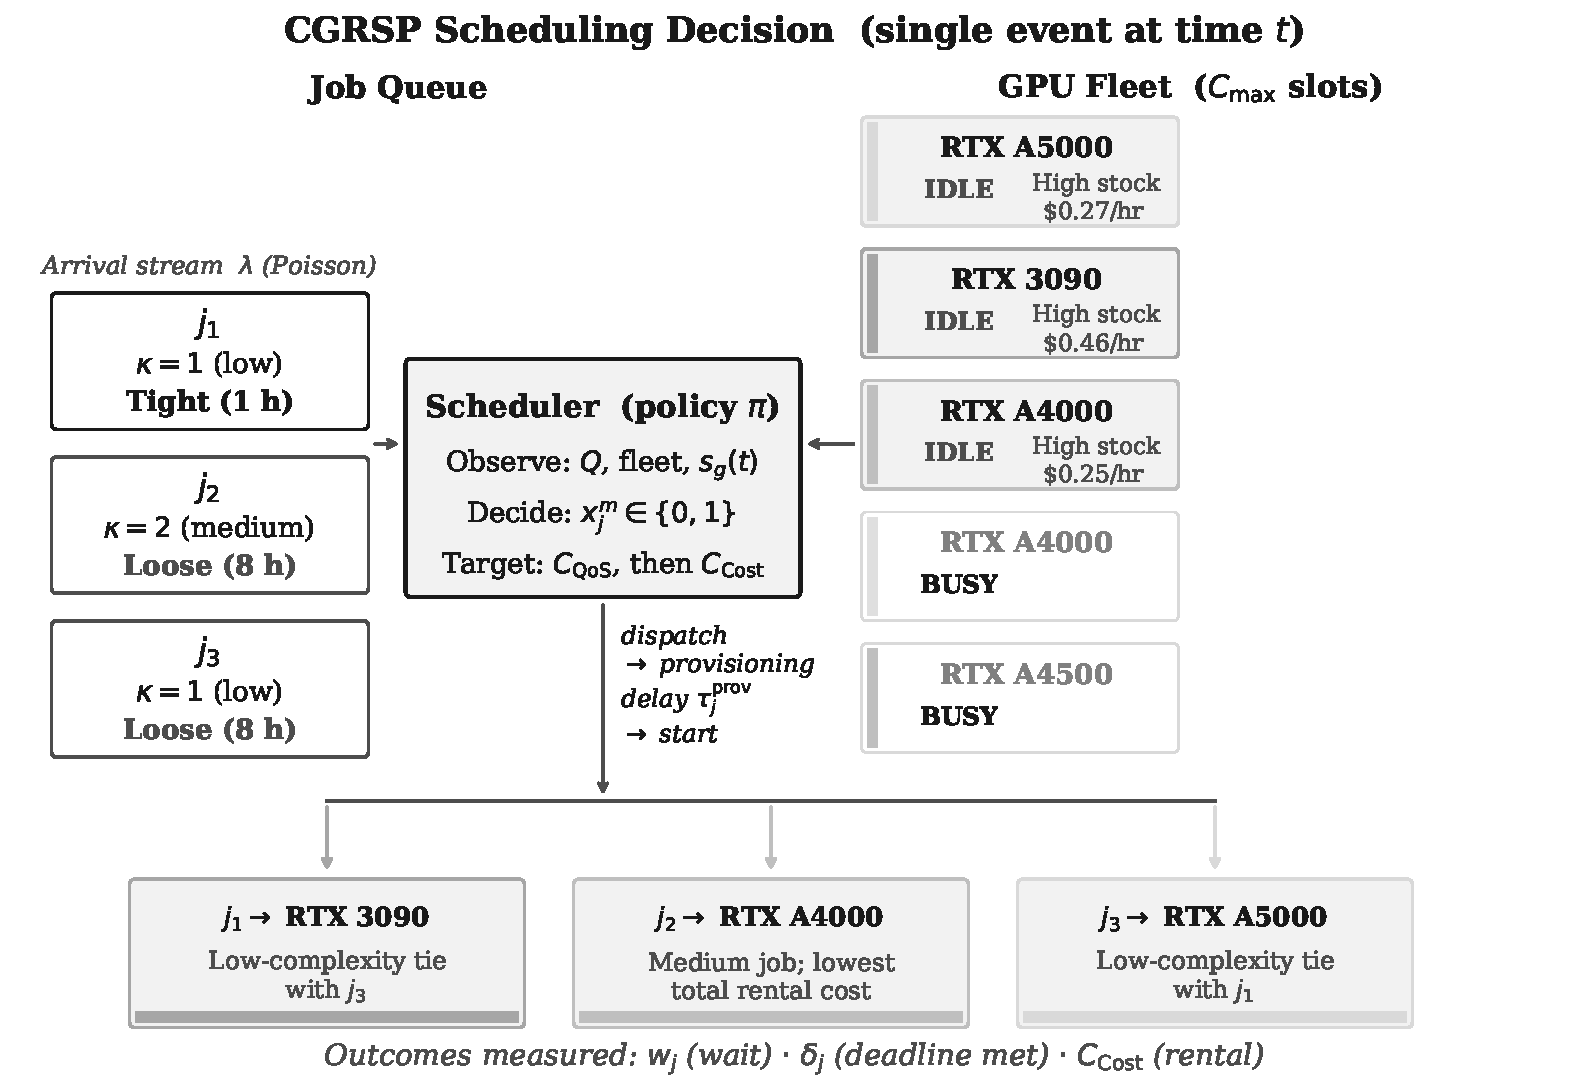
\includegraphics[width=0.98\linewidth,height=0.90\textheight,keepaspectratio]{figures/scheduling_decision.pdf}
\caption[CGRSP scheduling decision at a single event]{CGRSP scheduling decision at a single event.}
\label{fig:scheduling-decision}
\end{figure}
\end{landscape}

\noindent\textit{Figure~\ref{fig:scheduling-decision} notes.} CGRSP scheduling decision at a single event. The scheduler observes the job queue (jobs $j_1$--$j_3$ with complexity $\kappa$ and deadline class) and the GPU fleet ($C_{\max}$ slots with type, stock status, and occupancy). The diagram illustrates the formal lexicographic objective, QoS first (minimise the weighted wait and miss penalty), then cost as a tiebreaker; the implemented policies approximate it rather than solving the joint assignment exactly. The sketch assumes simultaneous dispatch at $t=0$, zero realised provisioning delay, and service times at their class means. Each job then has zero wait and meets its deadline on any of the three idle GPU types, so QoS ties. Minimising total rental cost over the complete assignment puts the medium job $j_2$ on the RTX~A4000 and the two low-complexity jobs on the RTX~3090 and A5000 in either order; the diagram shows one of these cost-tied placements. The tight deadline on $j_1$ does not require the fastest GPU while its one-hour window is non-binding. Busy slots (greyed) are unavailable. Dispatch incurs the provisioning delay $\tau_j^{\text{prov}}$ before a job starts running. The outcomes recorded per job are waiting time $w_j$, deadline adherence $\delta_j$, and rental cost.\par

\begin{table}[htbp]
\centering
\caption{System parameters}
\label{tab:parameters}
\begin{singlespace}
\small
\begin{tabular}{lp{9cm}}
\toprule
\textbf{Symbol} & \textbf{Description} \\
\midrule
$n_g$ & Number of nodes of resource type $g$ \\
$s_g(t)$ & Stock status of resource type $g$ at time $t$ (High / Medium / Low) \\
$p_g$ & Per-second rental price of resource type $g$ \\
$\lambda$ & Mean job arrival rate (jobs per second) \\
$\rho$ & Offered load, $\rho = \lambda\,\overline{W}/C_{\max}$, where $\overline{W}$ is the expected execution time averaged over the complexity mix and, with equal weight, over the $|\calG|$ resource types (not over the $C_{\max}$ slots) \\
$\kappa_j$ & Complexity level of job $j$ \\
$d_j$ & Deadline for job $j$ \\
$t_j^{\text{submit}}$ & Submission time of job $j$ \\
$W(j,g)$ & Realised execution time of job $j$ on resource type $g$; it depends on $j$ only through the complexity level $\kappa_j$, so the class-level form $W(\kappa_j, g)$ is used where convenient \\
$\overline{W}(\kappa,g)$ & Mean (expected) execution time of complexity class $\kappa$ on resource type $g$ \\
$\mu_{\kappa,g}, \sigma_{\kappa,g}$ & Log-space location and dispersion of the execution-time distribution of stratum $(\kappa,g)$; $\mu_{\kappa,g} = \ln \overline{W}(\kappa,g) - \tfrac{1}{2}\sigma_{\kappa,g}^2$ so that $\mathbb{E}[W(j,g)] = \overline{W}(\kappa_j,g)$ (Eq.~\ref{eq:servicetime}) \\
$\beta_g$ & Baseline high-stock probability of resource type $g$ \\
$\phi(t)$ & Time-of-day stock multiplier at time $t$ \\
$\tau^{\text{prov}}_j$ & Provisioning delay incurred when job $j$ acquires an instance (stock-status dependent) \\
$g(m)$ & Resource type of node $m$ \\
$g_j$ & Resource type of the node assigned to job $j$: $g(m)$ for the $m$ with $x_j^m = 1$ \\
$C_{\max}$ & Concurrency limit: number of on-demand slots ($|\calN| = C_{\max}$) \\
$L_s, U_s$ & Lower and upper provisioning-delay bounds for stock status $s$ \\
$p^{H}_g(t), p^{M}_g(t)$ & High-stock probability and Medium-band width (threshold increment) of resource type $g$ at time $t$ \\
$T_{\text{tight}},T_{\text{loose}}$ & Tight and loose deadline-window lengths (rush orders and standard renders); platform values and class proportions in Section~\ref{ssec:platform-and-data} \\
$T_j$ & Deadline window assigned to job $j$, $T_j \in \{T_{\text{tight}}, T_{\text{loose}}\}$ \\
$\alpha_1, \alpha_2$ & QoS penalty weights inside $C_{\text{QoS}}$: penalty per second of waiting ($\alpha_1$) and penalty per missed deadline ($\alpha_2$) \\
$w_{\text{qos}}, w_{\text{cost}}$ & Scalarisation weights balancing QoS and cost, used in the weighted-sum robustness variant (Section~\ref{ssec:objective-weight-sensitivity}) and in the Rolling-Horizon placement surrogate (Chapter~\ref{chap:system}) \\
\bottomrule
\end{tabular}
\end{singlespace}
\end{table}

\begin{table}[htbp]
\centering
\caption{Decision variables and state variables}
\label{tab:variables}
\begin{tabular}{lp{9cm}}
\toprule
\textbf{Symbol} & \textbf{Description} \\
\midrule
$x_j^m \in \{0,1\}$ & Assignment: 1 if job $j$ executes on node $m$ (realised placement over the horizon), 0 otherwise \\
$a_m^t \in \{0,1\}$ & Idle indicator for slot $m$ immediately before dispatch decisions at $t$, after completions at $t$ have released their slots (1 if free, 0 if still held by an earlier job) \\
$t_j^{\text{dispatch}}$ & Dispatch (slot-acquisition) time of job $j$: state variable determined by the scheduling policy \\
$t_j^{\text{start}}$ & Execution start time of job $j$ (Eq.~\ref{eq:starttime}) \\
$t_j^{\text{complete}}$ & Completion time of job $j$ \\
$w_j$ & Waiting time of job $j$ \\
$r_j$ & Response time of job $j$ \\
$\delta_j \in \{0,1\}$ & Deadline adherence indicator: 1 if job $j$ completes on time ($t_j^{\text{complete}} \leq d_j$), 0 otherwise \\
$\tau_j = \max(0, t_j^{\text{complete}} - d_j)$ & Tardiness of job $j$: auxiliary quantity (time past deadline, 0 if on time); defined for completeness, not part of the objective \\
$c_j$ & Execution cost of job $j$ (Eq.~\ref{eq:cost_cost}) \\
$\Delta_{\text{miss}}$ & Deadline miss rate: fraction of jobs that complete after their deadline (Eq.~\ref{eq:missrate}) \\
$C_{\text{QoS}}, C_{\text{Cost}}$ & QoS and operational-cost components of the lexicographic objective (Eqs.~\ref{eq:cqos} and~\ref{eq:ccost}) \\
\bottomrule
\end{tabular}
\end{table}

The system operates as a discrete-event simulator with continuous time representation. At each scheduling event, the scheduler observes the current state and makes assignment decisions. The state space includes both observable information and internal provisioning dynamics.

\textbf{Observable State (Scheduler View):} The scheduler receives a simplified three-state representation for each node:
\begin{itemize}
\item \textbf{Unavailable}: Slot cannot be rented. This state is retained for generality (it arises on a spot market); under the on-demand Secure Cloud model studied here a held slot is never reclaimed, so this state does not occur in the experiments.
\item \textbf{Idle}: Slot is free and can be assigned to jobs
\item \textbf{Running}: Slot is held by an assigned job, either being provisioned or executing
\end{itemize}
Additional observations: current job queue $\calJ_t$ with job characteristics $(\kappa_j, d_j, t_j^{\text{submit}})$, current simulation time $t$, and historical performance metrics.

In addition to per-node availability, the scheduler observes a per-type \textbf{stock status} $s_g(t) \in \{\text{High}, \text{Medium}, \text{Low}\}$ summarising the provisioning reliability of resource type $g$: the likelihood that a fresh instance of type $g$ can be acquired without a long provisioning delay. Stock status is distinct from the idle indicator $a_m^t$: $a_m^t$ records whether a held slot is currently free, whereas $s_g(t)$ reflects market-level scarcity of type $g$. Stock status governs the provisioning delay incurred when a fresh instance of type $g$ is acquired, formalised in Section~\ref{sec:mathematical-model}. In the simulator the status a scheduler observes and the status that fixes the realised delay are two independent draws from the same time-varying model, so the observation behaves as a stale poll rather than a binding quote (Section~\ref{ssec:platform-and-data}). Stock status also biases node selection (Chapter~\ref{chap:system}) away from scarce or unreliable types.

The fleet model enforces at most one job per node at any time: each provisioned instance is exclusively assigned to a single job until completion, and once started a job runs to completion without interruption, since checkpoint-restart mechanisms are expensive or unavailable for rendering workloads. While GPU virtualisation could enable multi-tenancy, the one-job-per-node restriction reflects common rendering workload requirements, where jobs use full GPU capacity for optimal performance.

The model assumes that the on-demand Secure Cloud pool makes every slot rentable at any time: the idle indicator $a_m^t \in \{0,1\}$ records only whether slot $m$ is currently free (1) or held by a job (0), and a held slot is never reclaimed by the provider. Market scarcity is therefore not realised as denial of service but as the provisioning delay $\tau^{\text{prov}}_j$ formalised in Section~\ref{sec:mathematical-model} (Eq.~\ref{eq:provdelay}); the delay ranges and stock-status parameters, stated as modelling assumptions informed qualitatively by the RunPod snapshot record, are given in Chapter~\ref{chap:experiments}.

\textbf{Human Decision Elements:} The formulation reflects human operational decisions through several design parameters:
\begin{itemize}
\item \textbf{Deadline policy}: Per-job deadline window from submission time ($d_j = t_j^{\text{submit}} + T_j$, where $T_j \in \{T_{\text{tight}}, T_{\text{loose}}\}$; values and class proportions are given in Section~\ref{ssec:platform-and-data})
\item \textbf{Fleet configuration} ($n_g$ for each $g \in \calG$): Capacity planning decision
\item \textbf{Deadline-penalty weights} ($\alpha_1, \alpha_2$): the business valuation of a missed deadline against accumulated waiting inside $C_{\text{QoS}}$; the scalar weights $w_{\text{qos}}, w_{\text{cost}}$ exist only in the robustness variant and the RH surrogate
\end{itemize}

\section{Mathematical Model}
\label{sec:mathematical-model}

The scheduling objective is bi-objective, with quality of service treated as the \emph{primary} criterion and operational cost as a \emph{secondary}, tiebreaking criterion. QoS is optimised first; operational cost is optimised only among assignments that are equivalent on QoS. This lexicographic priority is a modelling preference for service quality over rental spend, not a measured contractual penalty: the chosen $\alpha_2/\alpha_1=10$ equates one missed deadline with only ten seconds of waiting within the QoS component, as explained below. Formally, the model defines the following lexicographic objective; the online schedulers in Chapter~\ref{chap:system} use heuristics or surrogate scores rather than solving this joint optimisation exactly:
\begin{align}
\operatorname*{lex\,min}\; \bigl( C_{\text{QoS}},\; C_{\text{Cost}} \bigr) & \label{eq:objective}\\
C_{\text{QoS}} &= \sum_{j \in \calJ} \bigl[\, \alpha_1\, w_j + \alpha_2\, (1 - \delta_j) \,\bigr] \label{eq:cqos}\\
C_{\text{Cost}} &= \sum_{j \in \calJ} c_j \label{eq:ccost}
\end{align}
where lexicographic minimisation prefers any policy with lower $C_{\text{QoS}}$ and breaks QoS ties on lower $C_{\text{Cost}}$. The QoS cost (Eq.~\ref{eq:cqos}) combines a waiting-time penalty and a deadline-violation penalty: $w_j$ is the waiting time in seconds (Eq.~\ref{eq:wait}), $\alpha_1$ is the penalty per second of wait, and $\alpha_2$ is a penalty per missed deadline applied through the binary miss indicator $(1 - \delta_j)$. The concrete values of $\alpha_1$ and $\alpha_2$ used in experiments are given in Section~\ref{ssec:platform-and-data}; their ratio $\alpha_2/\alpha_1$ is swept in Section~\ref{ssec:objective-weight-sensitivity} to verify robustness. At the calibrated ratio $\alpha_2/\alpha_1 = 10$, one missed deadline is worth ten seconds of waiting, so the $C_{\text{QoS}}$ ordering of policies is essentially their mean-wait ordering; the headline ranking and the recommendations therefore use the miss rate $\Delta_{\text{miss}}$ directly rather than the scalar $C_{\text{QoS}}$. The cost criterion $C_{\text{Cost}}$ is the total rental spend across all provisioned instances, summing the per-job execution cost $c_j$, which is defined formally in Eq.~\ref{eq:cost_cost} below, once the assignment variable $x_j^m$ has been introduced through the constraints.

Subject to:
\begin{align}
\sum_{m \in \calN} x_j^m &= 1, & \forall j \in \calJ \label{eq:single_assign}\\
\sum_{j \in \calJ} x_j^m \, \mathbf{1}\!\left[t_j^{\text{dispatch}} \leq t < t_j^{\text{complete}}\right] &\leq 1, & \forall m \in \calN,\; \forall t \label{eq:single_job_node}\\
x_j^m &\leq a_m^{t_j^{\text{dispatch}}}, & \forall j \in \calJ,\; m \in \calN \label{eq:avail}
\end{align}
\begin{align}
p^{H}_g(t) &= \min\!\left(0.95,\, \beta_g\, \phi(t)\right), & p^{M}_g(t) &= \min\!\left(0.90,\, 1.5\,\beta_g\, \phi(t)\right), & \forall g \in \calG,\ \forall t \label{eq:stockprob}
\end{align}
\begin{equation}
\begin{gathered}
s_g(t) =
\begin{cases}
\text{High} & \text{if } u_{g,k} < p^{H}_g(t),\\
\text{Medium} & \text{if } p^{H}_g(t) \le u_{g,k} < p^{H}_g(t) + p^{M}_g(t),\\
\text{Low} & \text{otherwise},
\end{cases}\\[0.5ex]
\forall g \in \calG,\ \forall t,\quad u_{g,k} \overset{\text{i.i.d.}}{\sim} \text{Uniform}(0,1)\ \text{for the $k$-th draw made at time $t$}
\end{gathered}
\label{eq:stock}
\end{equation}
\begingroup
\allowdisplaybreaks
\begin{align}
W(j,g) &\sim \text{LogNormal}\!\left(\mu_{\kappa_j,g},\, \sigma_{\kappa_j,g}^2\right), & \forall j \in \calJ,\; g \in \calG \label{eq:servicetime}\\
\tau^{\text{prov}}_j &\sim \text{Uniform}\!\left(L_{\tilde s_{g_j}(t_j^{\text{dispatch}})},\; U_{\tilde s_{g_j}(t_j^{\text{dispatch}})}\right), & \forall j \in \calJ \label{eq:provdelay}\\
t_j^{\text{dispatch}} &\geq t_j^{\text{submit}}, & \forall j \in \calJ \label{eq:release}\\
t_j^{\text{start}} &= t_j^{\text{dispatch}} + \tau^{\text{prov}}_j, & \forall j \in \calJ \label{eq:starttime}\\
t_j^{\text{complete}} &= t_j^{\text{start}} + \sum_{m \in \calN} x_j^m W(j,g(m)), & \forall j \in \calJ \label{eq:completion}\\
d_j &= t_j^{\text{submit}} + T_j, & \forall j \in \calJ \label{eq:deadline_window}\\
w_j &= t_j^{\text{start}} - t_j^{\text{submit}}, & \forall j \in \calJ \label{eq:wait}\\
r_j &= t_j^{\text{complete}} - t_j^{\text{submit}}, & \forall j \in \calJ \label{eq:resp}\\
\tau_j &= \max(0,\, t_j^{\text{complete}} - d_j), & \forall j \in \calJ \label{eq:tardiness}\\
\delta_j &= \mathbf{1}[t_j^{\text{complete}} \leq d_j], & \forall j \in \calJ \label{eq:adherence}\\
\Delta_{\text{miss}} &= \frac{1}{|\calJ|}\sum_{j \in \calJ} (1 - \delta_j) \label{eq:missrate}\\
c_j &= \sum_{m \in \calN} x_j^m \, W(j, g(m))\, p_{g(m)}, & \forall j \in \calJ \label{eq:cost_cost}\\
x_j^m,\; a_m^t,\; \delta_j &\in \{0,1\},\ \ w_j,\, r_j,\, \tau_j,\, c_j \geq 0, & \forall j \in \calJ,\; m \in \calN,\; t \label{eq:domains}
\end{align}
\endgroup

Constraints~(\ref{eq:single_assign})--(\ref{eq:avail}) ensure feasible assignments respecting the concurrency limit and slot occupancy. The assignment variable $x_j^m$ records the realised placement over the whole horizon, so Constraint~(\ref{eq:single_job_node}) is stated per time instant using the indicator function $\mathbf{1}[\cdot]$, a standard piece of notation that evaluates to $1$ when the bracketed condition is true and $0$ otherwise. Concretely, $\mathbf{1}\!\left[t_j^{\text{dispatch}} \leq t < t_j^{\text{complete}}\right]$ equals $1$ exactly while node $m$ is held by job $j$, i.e.\ from its dispatch (the slot acquisition, so the provisioning window is included) up to (but not including) its completion time, and $0$ at every other instant. Multiplying by $x_j^m$ and summing over $j \in \calJ$ therefore counts how many jobs simultaneously hold node $m$ at instant $t$; bounding that count by $1$ states, in plain terms, that node $m$ can be held by at most one job at any given time, whether that job is still being provisioned or already executing. The half-open occupancy interval $[t_j^{\text{dispatch}}, t_j^{\text{complete}})$ inside the indicator lets a slot that completes a job at $t$ accept its successor at the same instant without double counting. Constraint~(\ref{eq:avail}) requires the chosen slot to be idle in the pre-decision state at the job's dispatch instant ($a_m^{t_j^{\text{dispatch}}} = 1$). Constraint~(\ref{eq:single_assign}) is a covering equality over the complete service horizon: every submitted job must eventually execute exactly once, and rejection is not allowed. This does not force immediate dispatch at an online event. An online policy uses only its observable state and history; the realised assignment variables describe its eventual schedule, not advance knowledge of the sampled service times. A job can remain in $\calJ_t$ until its chosen dispatch time; the realised horizon-wide placement $x_j^m$ is distinct from an event's decision to defer it. Constraint~(\ref{eq:release}) prevents dispatch before submission, while Equation~(\ref{eq:completion}) binds completion to execution start plus the realised service time on the assigned node. Since that service time is strictly positive, a job cannot occupy an empty interval or complete before starting. The concurrency limit $C_{\max}$ is encoded directly in $|\calN|$: the node set $\calN$ contains exactly $C_{\max}$ virtual on-demand slots, so at most $C_{\max}$ jobs can run simultaneously at any time $t$. Slots are costless when idle; rental charges apply only while a job is executing on one.

Equation~(\ref{eq:servicetime}) makes the realised execution time a log-normal random variable whose expectation is the stratum mean $\overline{W}(\kappa_j,g)$: the log-space location $\mu_{\kappa,g} = \ln \overline{W}(\kappa,g) - \tfrac{1}{2}\sigma_{\kappa,g}^2$ is fixed by that expectation, and the log-space dispersion $\sigma_{\kappa,g}$ is fitted per stratum in Chapter~\ref{chap:experiments}, so a job's expected duration is known at dispatch while its realised duration is not. Equations~(\ref{eq:stockprob}), (\ref{eq:stock}), (\ref{eq:provdelay}) and~(\ref{eq:starttime}) formalise the stochastic provisioning process that Section~\ref{sec:problem-description} introduced informally, made explicit here because the provisioning delay $\tau^{\text{prov}}_j$ it produces is a first-class component of the waiting time $w_j$, not an implementation detail. Each resource type $g$ carries a stock status $s_g(t)$ drawn by comparing one fresh uniform variate $u_{g,k} \sim \text{Uniform}(0,1)$, independent across types and across the draws $k$ made at successive dispatch events, against cumulative thresholds set by a baseline high-stock probability $\beta_g$ and a time-of-day multiplier $\phi(t)$; Equation~(\ref{eq:stockprob}) defines the two thresholds, capping the High-stock probability at $0.95$ and the Medium-band width at $0.90$, and Equation~(\ref{eq:stock}) draws the status from them. Because $p^{M}_g$ is the width of the Medium band and not the probability of Medium, the two thresholds are not clipped to a total of $1$: where $p^{H}_g + p^{M}_g \ge 1$ (for example the RTX~3090 in an off-peak hour, $0.65 + 0.90$) the draw never returns Low and the realised probability of Medium is $1 - p^{H}_g$; this is a deliberate property of the calibrated model and is disclosed with the availability assumptions in Section~\ref{ssec:platform-and-data}. When job $j$ is dispatched at time $t_j^{\text{dispatch}}$ to a slot of its assigned type $g_j$, it incurs the provisioning delay $\tau^{\text{prov}}_j$ drawn against a stock status $\tilde s_{g_j}(t_j^{\text{dispatch}})$ of that type at the dispatch instant, sampled from the same process as $s_g(t)$ but by an independent draw, so it need not equal the status the scheduler last observed (Eq.~\ref{eq:provdelay}), whose range depends on the stock status (per-status ranges in Section~\ref{ssec:platform-and-data}; the Low-state delays are orders of magnitude longer than High-state ones); the realised start time then follows from the dispatch time and this delay (Eq.~\ref{eq:starttime}), so $\tau^{\text{prov}}_j$ forms a component of the waiting time $w_j$ (Eq.~\ref{eq:wait}). The $\beta_g$ values, the $\phi(t)$ bands, and the resulting frequency of each stock state are parameter values given in Chapter~\ref{chap:experiments}, where they are stated as modelling assumptions rather than empirical frequencies.

Equation~(\ref{eq:deadline_window}) fixes each job's absolute deadline from its per-job deadline window $T_j$. Unlike hard-deadline models, the CGRSP formulation treats deadlines as soft: violations are penalised in the objective rather than structurally prohibited. This reflects operational reality under the $C_{\max}$ concurrency ceiling: when the offered load $\rho = \lambda\,\overline{W}/C_{\max}$ exceeds one the queue tends to grow for as long as the arrival burst lasts, and with online arrivals, stochastic provisioning delays and stochastic service times some misses are then a routine outcome of real operation even where capacity alone forces none (on the hectic day the window-capacity bound of Section~\ref{ssec:capacity-lower-bound} certifies zero unavoidable misses). A penalty formulation that grades misses, rather than a hard constraint that would declare such realisations infeasible, is therefore the appropriate model.

Equations~(\ref{eq:wait})--(\ref{eq:adherence}) define the QoS metrics tracked for each job. Equation~(\ref{eq:missrate}) aggregates the per-job indicators into the deadline miss rate $\Delta_{\text{miss}}$, the fraction of jobs that complete after their deadline; it is the primary QoS statistic reported in Chapter~\ref{chap:experiments}. The response time $r_j$ (Eq.~\ref{eq:resp}) is the job's total sojourn from submission to completion, the sum of its waiting time $w_j$ and its realised execution time; it does not enter the objective and is tracked as a diagnostic, reported in Chapter~\ref{chap:experiments} through those two components rather than as a separate column. Figure~\ref{fig:job-lifecycle} illustrates how each interval maps onto a job's timeline for both the on-time and the missed-deadline cases. Deadline violations are penalised in the objective via the binary miss indicator $(1 - \delta_j)$ rather than via continuous tardiness $\tau_j$; tardiness (Eq.~\ref{eq:tardiness}) is defined for completeness but is not used in the objective. The miss-indicator form is the appropriate QoS penalty in a rendering-studio context because a missed client deadline is a discrete, qualitatively costly event (contract penalties, pipeline delays) rather than a quantity that scales with how late the job is; once a job will miss, its exact lateness is of secondary operational concern, so the objective penalises whether a deadline is met, not by how much. A corollary is that the scheduler should not sacrifice jobs that can still be saved in order to reduce the lateness of jobs that are already doomed. Mean tardiness is nonetheless reported as a diagnostic metric in Chapter~\ref{chap:experiments}, because the severity of missed deadlines matters operationally even when the count of misses is the primary objective. A robustness study (Chapter~\ref{chap:experiments}, Section~\ref{ssec:objective-weight-sensitivity}) re-scores a six-policy subset (FIFO, SPT, EDF, SPT+Rescue, RH and CADR) against a tardiness-based objective, and the per-metric leaders within that subset are unchanged: RH retains the lowest miss-rate point estimate and CADR attains the lowest mean tardiness on that ten-seed re-scoring set (at the 30-seed Phase~3 scale EDF's tardiness is marginally lower, Table~\ref{tab:statistical}). The subset boundary matters and is stated explicitly here, because that study omits the Adaptive EDF-SPT hybrid, which records a lower mean tardiness than CADR in the full ten-scheduler comparison (Section~\ref{sec:phase-3-statistical-validation}) while matching neither proposed scheduler on miss rate; CADR is therefore the lowest-tardiness policy of the re-scored six on that set, not of the fleet of policies evaluated in this thesis. What the tardiness objective does shift is the single scalarised winner, which moves towards low-tardiness policies; the decomposed conclusions of this thesis are therefore robust to the deadline-penalty form, while any single collapsed score is not.

\begin{landscape}
\begin{figure}[H]
\centering
\captionsetup{font=small,skip=6pt}
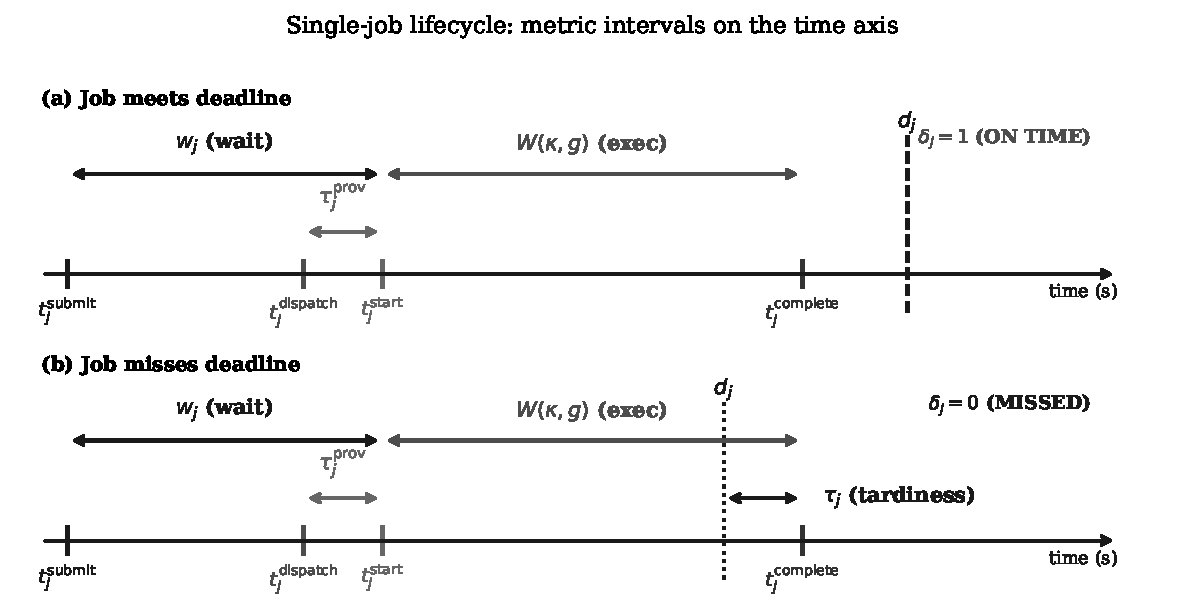
\includegraphics[width=0.98\linewidth,height=0.72\textheight,keepaspectratio]{figures/job_lifecycle.pdf}
\caption[Single-job lifecycle and metric intervals]{Single-job lifecycle: metric intervals mapped onto the time axis. Panel~(a) shows a job that meets its deadline ($\delta_j=1$): the waiting time $w_j$ spans submission to execution start and includes the provisioning delay $\tau^{\text{prov}}_j$ incurred between dispatch ($t_j^{\rm dispatch}$, slot acquisition) and execution start ($t_j^{\rm start}$); the execution time $W(\kappa,g)$ then runs to completion before the deadline $d_j$. Panel~(b) shows a missed deadline ($\delta_j=0$): completion falls after $d_j$, and tardiness $\tau_j = t_j^{\rm complete} - d_j > 0$.}
\label{fig:job-lifecycle}
\end{figure}
\end{landscape}

Equation~(\ref{eq:cost_cost}) defines the per-job execution cost $c_j$ that Eq.~\ref{eq:ccost} sums over $\calJ$ into the operational cost component $C_{\text{Cost}}$: the per-second rental fees for the provisioned GPU instances across all nodes, where $W(j, g(m))$ is the realised execution time of job $j$ on the assigned node's type (the stochastic execution-time model is calibrated in Chapter~\ref{chap:experiments}). Note the asymmetry in how the provisioning delay is accounted: $\tau^{\text{prov}}_j$ counts fully towards the waiting time $w_j$ (Eqs.~\ref{eq:starttime} and~\ref{eq:wait}) and hence towards the QoS penalty, but it is \emph{not} billed, since rental charges accrue only over the execution interval $[t_j^{\text{start}}, t_j^{\text{complete}}]$; a scarce GPU type therefore hurts the scheduler through QoS, not through cost. Finally, Constraint~(\ref{eq:domains}) states the natural domains of the decision and state variables.

Because the value of a missed deadline relative to accumulated waiting (the ratio $\alpha_2/\alpha_1$) is a business policy rather than a physical constant, no single value is canonical; the deadline-penalty ratio is swept in the objective-weight sensitivity analysis (Section~\ref{ssec:objective-weight-sensitivity}), which additionally evaluates a fully symmetric weighted-sum scalarisation $\min \bigl[\, w_{\text{qos}}\, C_{\text{QoS}} + w_{\text{cost}}\, C_{\text{Cost}} \,\bigr]$ with $w_{\text{qos}} = w_{\text{cost}} = 0.5$ as a robustness variant. Although RH wins the tested binary-miss grid, a symmetric scalar can in general let a small cost difference reorder policies separated on QoS; the lexicographic objective avoids this by construction, which is why all headline comparisons are reported on the decomposed metrics (mean wait, miss rate, and cost) rather than on a scalar value.

\section{Modelling Simplifications and Assumptions}
\label{sec:modelling-simplifications-and-assumptions}

The formulation rests on five modelling simplifications, collected here so that the assumptions behind every later result are stated once in one place rather than reconstructed from the simulator design (Chapter~\ref{chap:system}) or from the experimental chapters that follow. Each remark states the simplification, why it is defensible for the rendering workload studied, and what relaxing it would require.

\begin{enumerate}
\item \textbf{Remark 1, stochastic execution times.} The realised execution time $W(j,g)$ is a random variable, not a constant fixed by the pair (complexity level, resource type). It is drawn from the per-stratum log-normal service-time model of Equation~(\ref{eq:servicetime}), whose expectation is the stratum mean $\overline{W}(\kappa_j, g)$ and whose dispersion parameters are fitted in Chapter~\ref{chap:experiments}. What the pair does fix is that expectation, so a job's realised duration is uncertain while its expected duration is known: schedulers plan with $\overline{W}(\kappa_j, g)$ and observe the realised value only on completion, mirroring a dispatcher that can classify a scene's complexity before rendering but cannot know its exact walltime. Relaxing this towards heavier-tailed or correlated service times would change the variance of the QoS metrics rather than the structure of the model.

\item \textbf{Remark 2, one job per node.} Constraint~(\ref{eq:single_job_node}) admits at most one job holding a node at any instant, from dispatch to completion, so a provisioned instance is held exclusively for the duration of its job. This reflects rendering practice, where a job consumes the full GPU for best performance, and it is what makes the concurrency ceiling $C_{\max}$ a meaningful capacity limit. GPU virtualisation would permit multi-tenancy and would require a per-node resource-share variable in place of the binary $x_j^m$.

\item \textbf{Remark 3, no preemption.} Once execution begins, a job runs to completion without interruption, migration, or restart, because checkpoint-restart is expensive or unavailable for rendering pipelines. A consequence used throughout the scheduler designs is that a placement decision is irrevocable for the length of the job, so anticipation must happen before dispatch rather than through later correction.

\item \textbf{Remark 4, Poisson arrivals.} Jobs arrive as a Poisson process with mean rate $\lambda$, that is, with independent, memoryless, exponentially distributed inter-arrival times, the canonical model for independent submissions from separate clients and scenes. The day-type values of $\lambda$ used in the experiments are set in Chapter~\ref{chap:experiments}. Bursty or self-similar arrival processes would raise queueing delay at the same mean rate and are not modelled here.

\item \textbf{Remark 5, binary availability.} The idle indicator satisfies $a_m^t \in \{0,1\}$, so the scheduler observes a definite idle or running status for every slot rather than a partial or probabilistic one. Market scarcity is not modelled as denial of service under the on-demand Secure Cloud pool studied here, since a held slot is never reclaimed; it enters instead through the stochastic provisioning delay $\tau^{\text{prov}}_j$ of Eq.~(\ref{eq:provdelay}), which is itself driven by the per-type stock status $s_g(t)$ of Eq.~(\ref{eq:stock}). A spot-market variant would restore the Unavailable state of Section~\ref{sec:problem-description} and make availability itself stochastic.
\end{enumerate}

\section{Numerical Example}
\label{sec:numerical-example}

A minimal three-job, two-GPU instance makes the interplay of constraints visible. Two resource types are in the fleet: an RTX~3090 ($g_1$) and an RTX~A4000 ($g_2$). The concurrency cap is $C_{\max}$ (five slots in the experimental platform, Section~\ref{ssec:platform-and-data}); only three are used here, leaving two idle. Slots $m_2$ and $m_3$ are RTX~A4000 slots; $m_1$, $m_4$ and $m_5$ are RTX~3090 slots. Three jobs $\calJ = \{j_1, j_2, j_3\}$ arrive simultaneously at $t = 0$; nodes begin available ($a_m^0 = 1$ for all $m \in \calN$), and every resource type starts at High stock ($s_g(0) = \text{High}$).

\textbf{Job Characteristics:}
\begin{center}
\begin{tabular}{llll}
\toprule
\textbf{Job}&\textbf{Complexity}&\textbf{Submit Time}&\textbf{Deadline}\\
\midrule
$j_1$&$\kappa = 1$ (Low)&$t=0$&$t=3600$ (tight)\\
$j_2$&$\kappa = 2$ (Medium)&$t=0$&$t=28800$ (loose)\\
$j_3$&$\kappa = 1$ (Low)&$t=0$&$t=28800$ (loose)\\
\bottomrule
\end{tabular}
\end{center}

\textbf{Expected Execution Times} $\overline{W}(\kappa, g)$ (seconds; realised times are taken at their expected values in this example; see Table~\ref{tab:gpu_specs} for full GPU specifications):
\begin{center}
\begin{tabular}{lcc}
\toprule
\textbf{Complexity}&\textbf{RTX 3090 ($g_1$)}&\textbf{RTX A4000 ($g_2$)}\\
\midrule
Low ($\kappa=1$)&59.5&63.3\\
Medium ($\kappa=2$)&69.6&72.1\\
High ($\kappa=3$)&91.2&98.6\\
\bottomrule
\end{tabular}
\end{center}

Figure~\ref{fig:numerical-example} illustrates the assignment and timeline.

\begin{landscape}
\begin{figure}[H]
\centering
\captionsetup{font=small,skip=6pt}
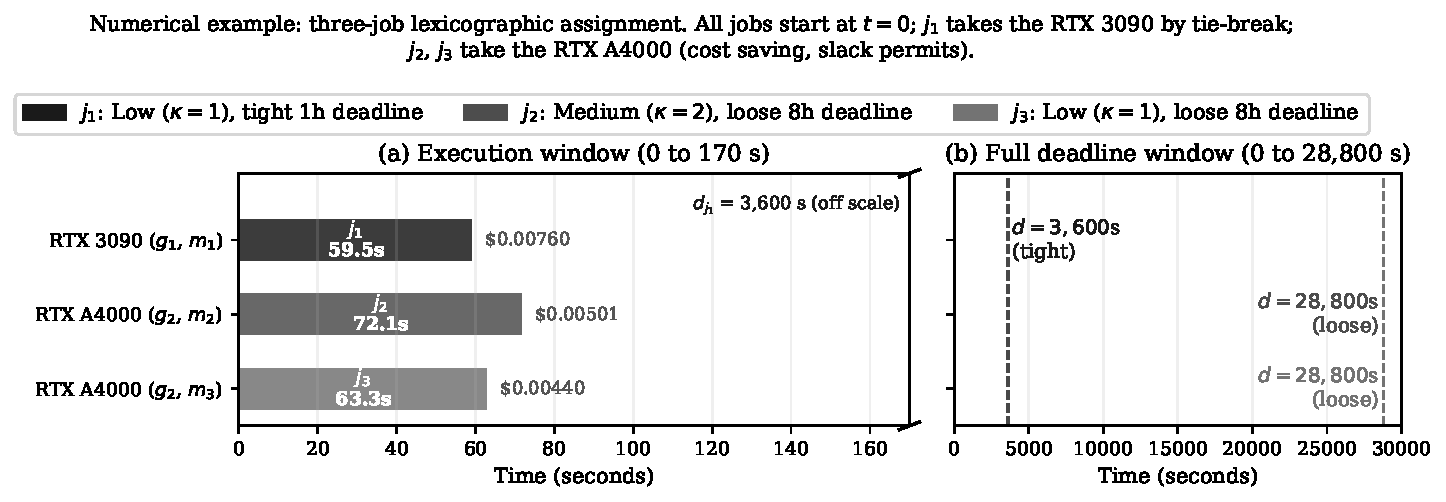
\includegraphics[width=0.98\linewidth,height=0.72\textheight,keepaspectratio]{figures/numerical_example.pdf}
\caption[Numerical example: three-job schedule on two GPUs]{Visual aid for the three-job numerical example. (a)~Execution window: all three jobs start immediately (High stock, negligible provisioning delay). $j_1$ (dark grey) runs on the RTX~3090 for 59.5\,s; $j_2$ (mid grey) and $j_3$ (light grey) run concurrently on separate RTX~A4000 slots for 72.1\,s and 63.3\,s respectively. Dollar annotations show per-job cost. The tight deadline $d_{j_1}=3{,}600$\,s is indicated by a dashed black line. (b)~Full deadline window: $j_2$ and $j_3$ each have an 8-hour loose deadline (28{,}800\,s), vastly exceeding their execution times and confirming that cost is the only discriminating criterion for those two jobs.}
\label{fig:numerical-example}
\end{figure}
\end{landscape}

\textbf{Assignment under the lexicographic objective.}
Every job here starts at $t=0$ and finishes within about a minute, so all three meet their deadlines with zero waiting on either GPU type. This includes $j_1$, whose one-hour window does not bind at this load. The three jobs are therefore QoS-equivalent across the fleet, since $w_j$ (Eq.~\ref{eq:wait}) excludes execution time, and the secondary cost criterion decides every placement. The A4000 saving is largest for the medium job, so $j_2$ takes one of the two RTX~A4000 slots. The other goes to a low-complexity job, and the remaining low-complexity job takes an RTX~3090 slot. Because $j_1$ and $j_3$ cost the same there, the objective leaves a tie, broken here in favour of the tight job ($x_{j_1}^{m_1} = x_{j_2}^{m_2} = x_{j_3}^{m_3} = 1$). Note that $j_2$'s medium complexity creates no tension here, whichever GPU is faster: both A4000 means used above rest on the relative-performance estimate, because the medium-complexity A4000 cell has only $n=2$ observed jobs (below the reliability threshold; their raw mean is 73.1\,s, against 69.6\,s for the RTX~3090, while the estimate is 72.1\,s) and there is no observed low-complexity A4000 job at all. Even if the RTX~3090 is faster in a stratum, eight hours of slack would strip that speed advantage of any QoS value and the cost tiebreaker would still prevail. The two remaining slots are left idle ($x_j^{m_4} = x_j^{m_5} = 0$ for every $j$).

\textbf{Outcome.}
All three jobs start immediately: every type begins at High stock, where the provisioning delay (Eq.~\ref{eq:provdelay}) is at most 10\,s (Section~\ref{ssec:platform-and-data}) and is taken as zero here, so every waiting-time penalty is zero ($w_{j_1} = w_{j_2} = w_{j_3} = 0$~s) and all deadlines are met (the QoS objective is at its optimum). Rental cost then works out to
$59.5 \times 0.000128 + 72.1 \times 0.0000694 + 63.3 \times 0.0000694 = \$0.017$,
where the per-second rates are derived from the RTX~3090 price of \$0.46/hr and the RTX~A4000 price of \$0.25/hr (Table~\ref{tab:gpu_specs}). Fleet utilisation is $3/5 = 60\%$. The key observation is that at this load every cost saving comes at no QoS penalty. Only once waiting or provisioning delay began to threaten $j_1$'s one-hour window would its tight deadline override cost. This ordering, QoS first and cost only among QoS-equivalent options, drives the scheduler designs described in Chapter~\ref{chap:system}.
